\DiaryEntry{Distance between (Random) Points on Lines}{2016-07-11}{Stochastic}

\subsection{Expected Distance between a fixed Point and a random Point on a Line}

Consider the one-dimensional problem of a point P at \(x=0\) and a line
\(x=L \ldots L+1\). Now choose a random point in uniform fashion on the
line. Let \(d\) denote the random distance between P and the randomly
chosen point. The Figure below shows the problem geometry.

\begin{figure}[H]
\centering

\includegraphics[scale=0.7]{images/expected_distances_01_01.png}
\end{figure}

We want to calculate the expected value of \(d\):

\[
\mathbb{E}(d) = \int_{x=L}^{L+1} x dx = \left. \frac{x^2}{2} \right|_{x=L}^{L+1} = \frac{1}{2} \left[ (L+1)^2 - L^2 \right] = L + 1/2
\]

which is somehow what we expected.

If we consider the expected value of the \emph{squared} distance, we
arrive at

\[
\mathbb{E}(d^2) = \int_{x=L}^{L+1} x^2 dx = \left. \frac{x^3}{3} \right|_{x=L}^{L+1} = \frac{L^3 + 3L^2 + 3L + 1 - L^3}{3} = L(L+1) + \frac{1}{3}
\]

which does not look overly intuitive\ldots{} If we compare
\((\mathbb{E}(d))^2\) and \(\mathbb{E}(d^2)\), we see that
\((\mathbb{E}(d))^2\) is always smaller:

\bee
(L+\frac{1}{2})^2 \leq L(L+1)+\frac{1}{3} \rightarrow L^2 + L + \frac{1}{4} \leq L^2 + L + \frac{1}{3} \rightarrow \frac{1}{4} \leq \frac{1}{3}
\eee

This is due to Jensen's Inequality: For any convex function \(\phi\), we
have \(\phi(\mathbb{E}(X)) \leq \mathbb{E}(\phi(X))\). Since \(()^2\) is
a convex function, the inequality holds.

Also interesting is the fact, that the difference between the two
expectations is constant and independent of L:
\(\mathbb{E}(d^2) - (\mathbb{E}(d))^2 = 1/12\).

\subsection{Expected Distance between two random Points on a Line
(I)}\label{expected-distance-between-two-random-points-on-a-line-i}

Now consider two lines; one at \(x=0 \ldots 1\) and one at
\(x=L \ldots L+1\) with \(L \geq 1\). The Figur below shows the problem
geometry.

\begin{figure}
\centering
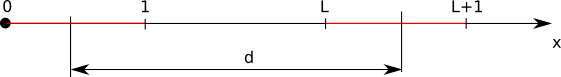
\includegraphics[scale=0.7]{images/expected_distances_01_02.png}
\end{figure}

The expected value of \(d\) is obtain as

\[
\mathbb{E}(d) = \int_{x_2=L}^{L+1} \int_{x_1=0}^{1} x_2 - x_1 dx_1 dx_2
\]

There seems to be no clever trick than to brute force evaluate the
integral. For the inner integral, we obtain

\[
\int_{x_1=0}^{1} x_2 - x_1 dx_1 = \left. x_1 x_2 - \frac{x_1^2}{2} \right|_{x_1=0}^1 = x_2 - \frac{1}{2}
\]

Inserting this into the outer integral, we obtain

\[
\mathbb{E}(d) = \int_{x_2=L}^{L+1} x_2 - \frac{1}{2} dx_2 = \left. \frac{x_2^2}{2} - \frac{x_2}{2} \right|_{x_2=L}^{L+1} = \cdots = L
\]

which is again what we expected.

If we perform the same exercise for the squared distance, we arrive at

\[
\mathbb{E}(d) = \int_{x_2=L}^{L+1} \int_{x_1=0}^{1} (x_2 - x_1)^2 dx_1 dx_2 = \ldots = L^2 + \frac{1}{6}
\]

As above, we have \((\mathbb{E}(X))^2 \leq \mathbb{E}(X^2)\); and again
we have the interesting fact, that the difference between the two terms
is constant and independent of L.

\subsubsection{Overlapping Lines}

In the special case that both lines overlap; i.e.~both lines range from
\(0\) to \(1\), we need to consider the absolute value of the distance:

\bee
\mathbb{E}(|d|) = \int_{x_2=0}^1 \int_{x_1=0}^1 |x_2 - x_1| dx_1 dx_2
\eee

We can get rid of the absolute value in the integral if we split the
integration:

\bee
\mathbb{E}(|d|) = \int_{x_2=0}^1 \left( \int_{x_1=0}^x2 x_2 - x_1 dx_1  +  \int_{x_1=x_2}^1 x_1 - x_2 dx_1 \right) dx_2
\eee

The integration is tedious, but standard and yields
\(\mathbb{E}(|d|) = 1/3\).
\href{http://math.stackexchange.com/questions/195245/average-distance-between-random-points-on-a-line}{Here}
is also a discussion of the problem; there are also several attempts to
provide the intuition behind the answer.

In case we drop the absolute value we obtain \(\mathbb{E}(d) = 0\). This
seems plausible as the problem is symmetric: For any pair \((x_1,x_2)\),
the integral will contain a contribution for \(x_2 - x_1\) and
\(x_1 - x_2\). They will have the same probability but different sign
and will therefore cancel out.

\subsection{Expected Distance between two random Points on a Line (II)}

If the lines are spaced apart in the y-direction, we can also evalulate
the mean (squared) distance. The problem geometry is shown below.

\begin{figure}
\centering
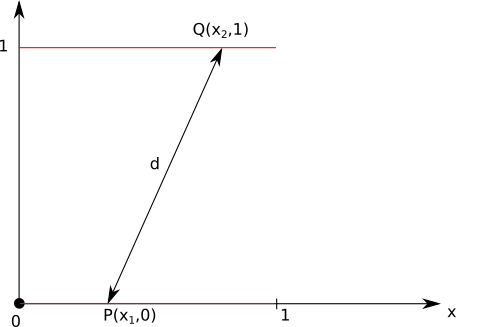
\includegraphics[scale=0.7]{images/expected_distances_01_03.png}
\end{figure}

The distance d between the points P and Q is given by
\(d = \sqrt{(x_2 - x_1)^2 + 1}\) and we obtain for the (simpler)
expected value of the squared distance

\bee
\mathbb{E}(d^2) = \int_{x_2=0}^1 \int_{x_1=0}^1 (x_2 - x_1)^2 + 1 dx_1 dx_2 = \ldots = \frac{7}{6}
\eee

If we are interested in the expected distance itself, we have to solve
the integral

\bee
\mathbb{E}(d^2) = \int_{x_2=0}^1 \int_{x_1=0}^1 \sqrt{(x_2 - x_1)^2 + 1} dx_1 dx_2 = \ldots = \frac{2-\sqrt{2}}{3} - \log \left( 1 + \sqrt{2} \right)
\eee

but I do not know how sympy was able to solve this integral.
